% vim:ft=tex

\section{Task Description}\label{tasks}

The first part can be roughly divided into two parts:
\begin{enumerate}
\item Data Engineering
\begin{itemize}
\item Data Profiling
\item identify potential difficulties
\item store data set
\end{itemize}
\item Virtual Infrastructure
\begin{itemize}
\item install and configure Nominatim
\item install and evaluate different Hadoop distributions
\end{itemize}
\end{enumerate}
The project should be implemented in an agile manner, therefore we will follow the development process of \textbf{Scrum}. This allows flexibility during the project in terms of specific tasks and topics.
\\\\
To gain a better understanding of the project and its goals we created a \glqq Big Picture\grqq of the applied technologies and the relations among themselves which can be seen in figure \ref{fig:big}.

\begin{figure}[H]
\hspace{-0.9cm}
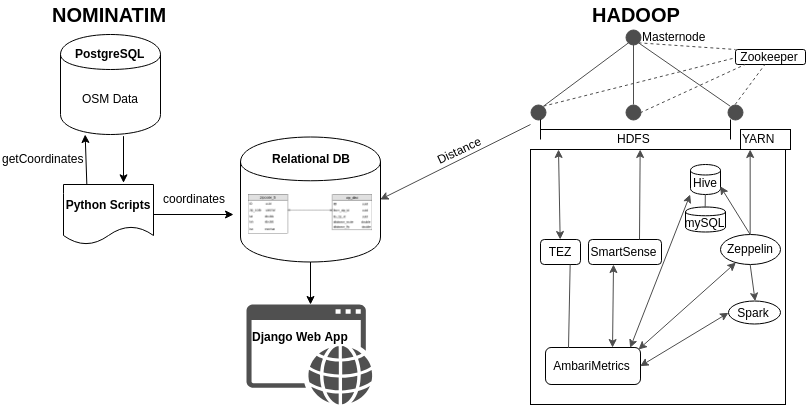
\includegraphics[width=1.1\textwidth]{img/big}
\captionof{figure}{Overview of project architecture}\label{fig:big}
\end{figure}
\noindent According to this picture the project can be classified more detailed into four parts:
\begin{enumerate}
\item Nominatim
\item Hadoop
\item Database
\item WebApp
\end{enumerate}
The implementation of those four parts will be documented in the following chapters.
